\documentclass{article}
\usepackage{main}

% Aquí empieza el documento{{{
\begin{document}

%\maketitle
\textbf{Alberto Oporto Ames \#139}
\thispagestyle{fancy}

% Fotos {{{
\begin{figure}[h]
	\begin{subfigure}{0.48\textwidth}
		\centering
		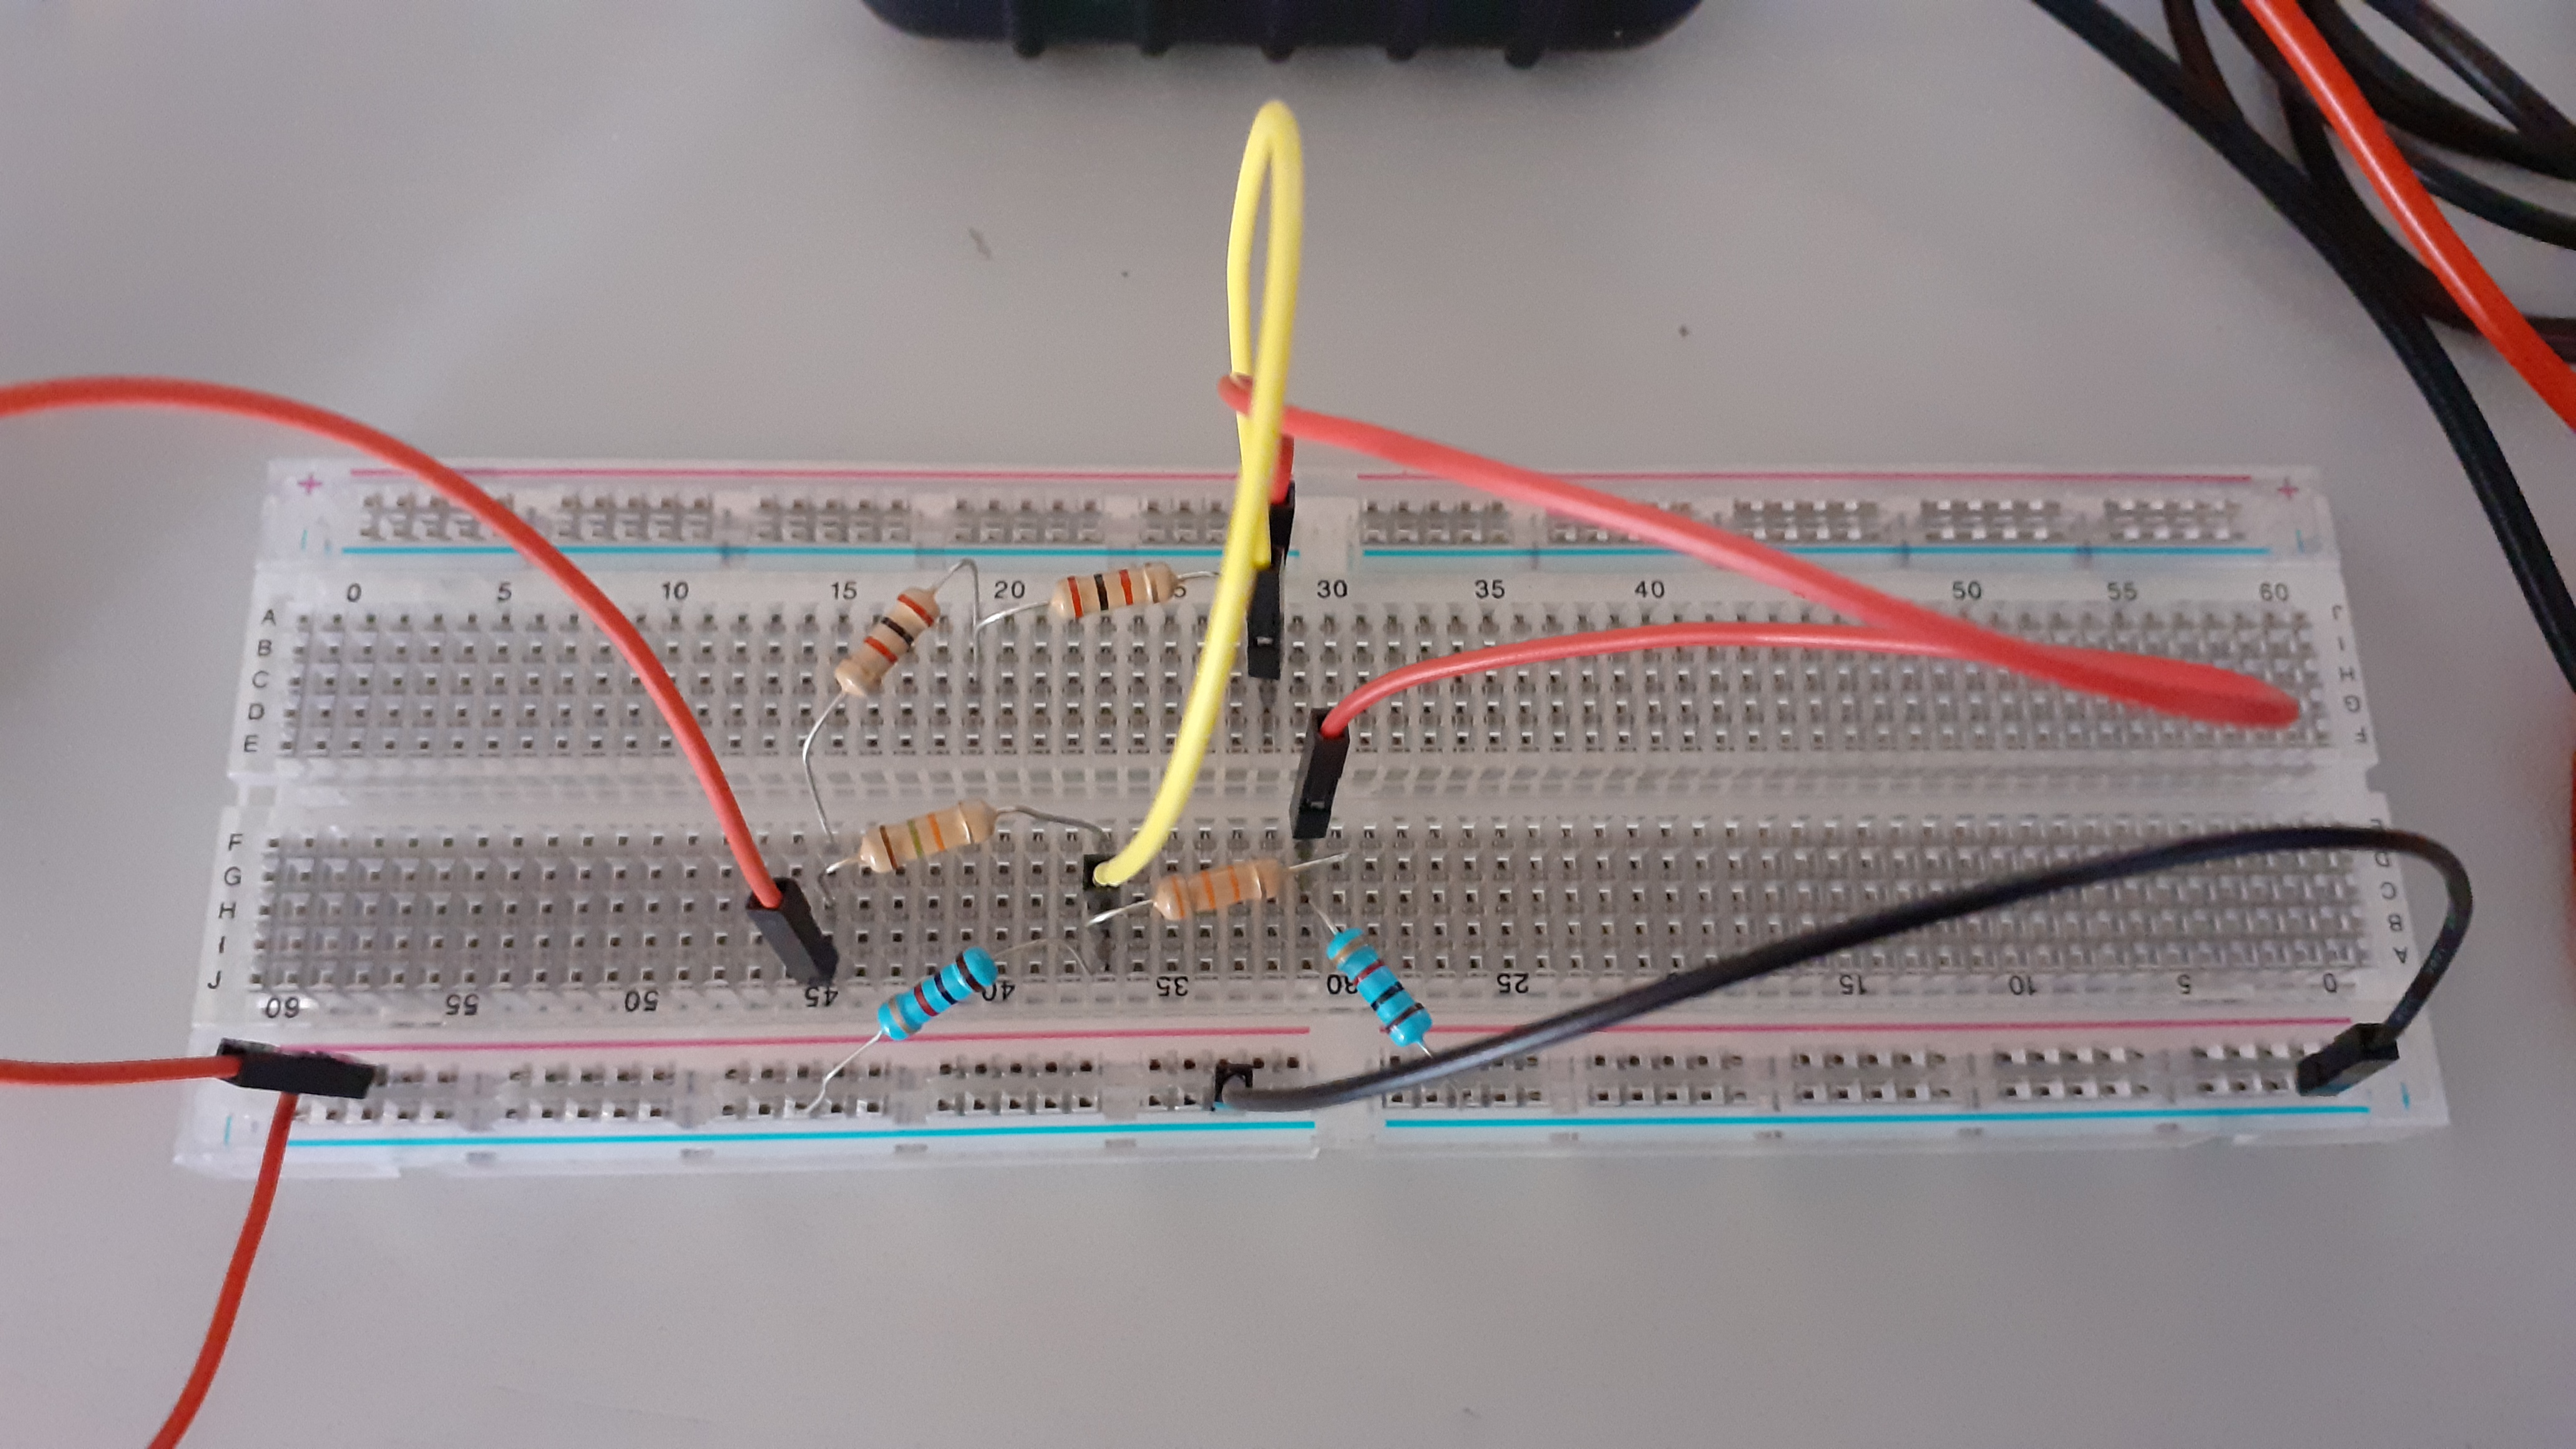
\includegraphics[width=0.9\linewidth]{20191108_092649}
		\caption{Circuito}%
		\label{fig:circuito}
	\end{subfigure}
	\begin{subfigure}{0.48\textwidth}
		\centering
		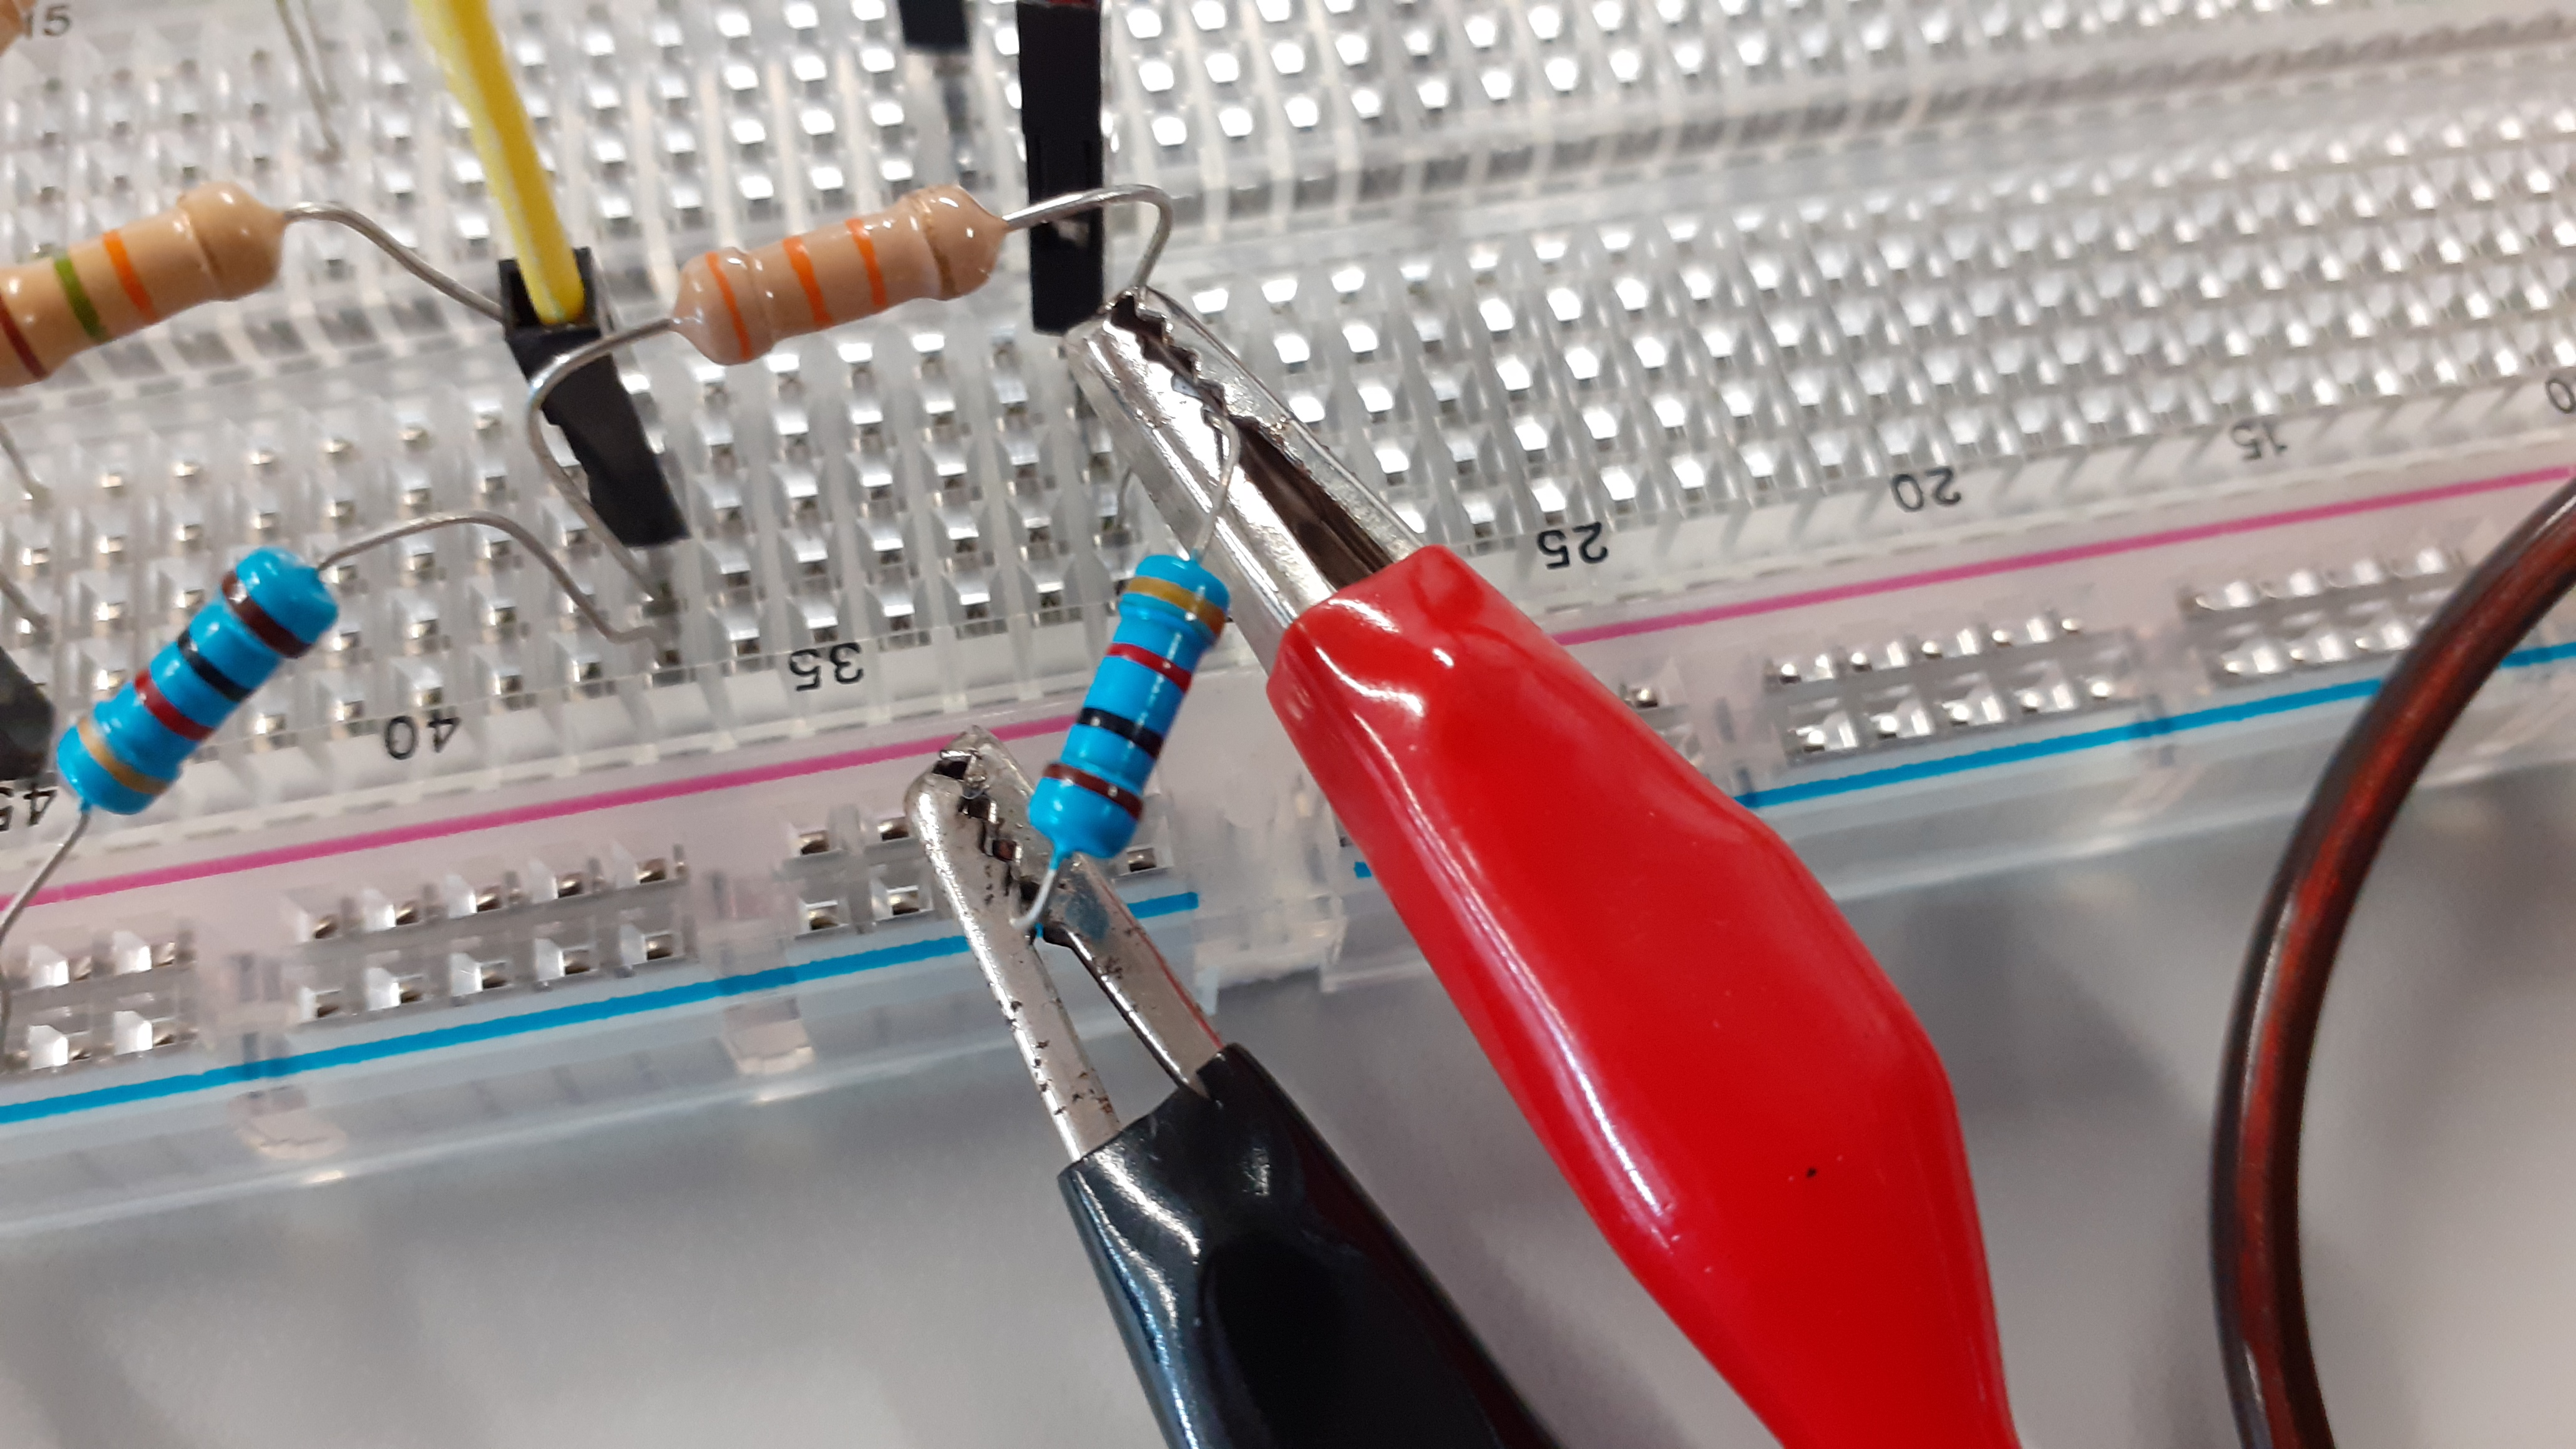
\includegraphics[width=0.9\linewidth]{20191108_093211}
		\caption{$V_1$}%
		\label{fig:v1}
	\end{subfigure}

	\vspace{0.5cm}
	\centering
	\begin{subfigure}{0.48\textwidth}
		\centering
		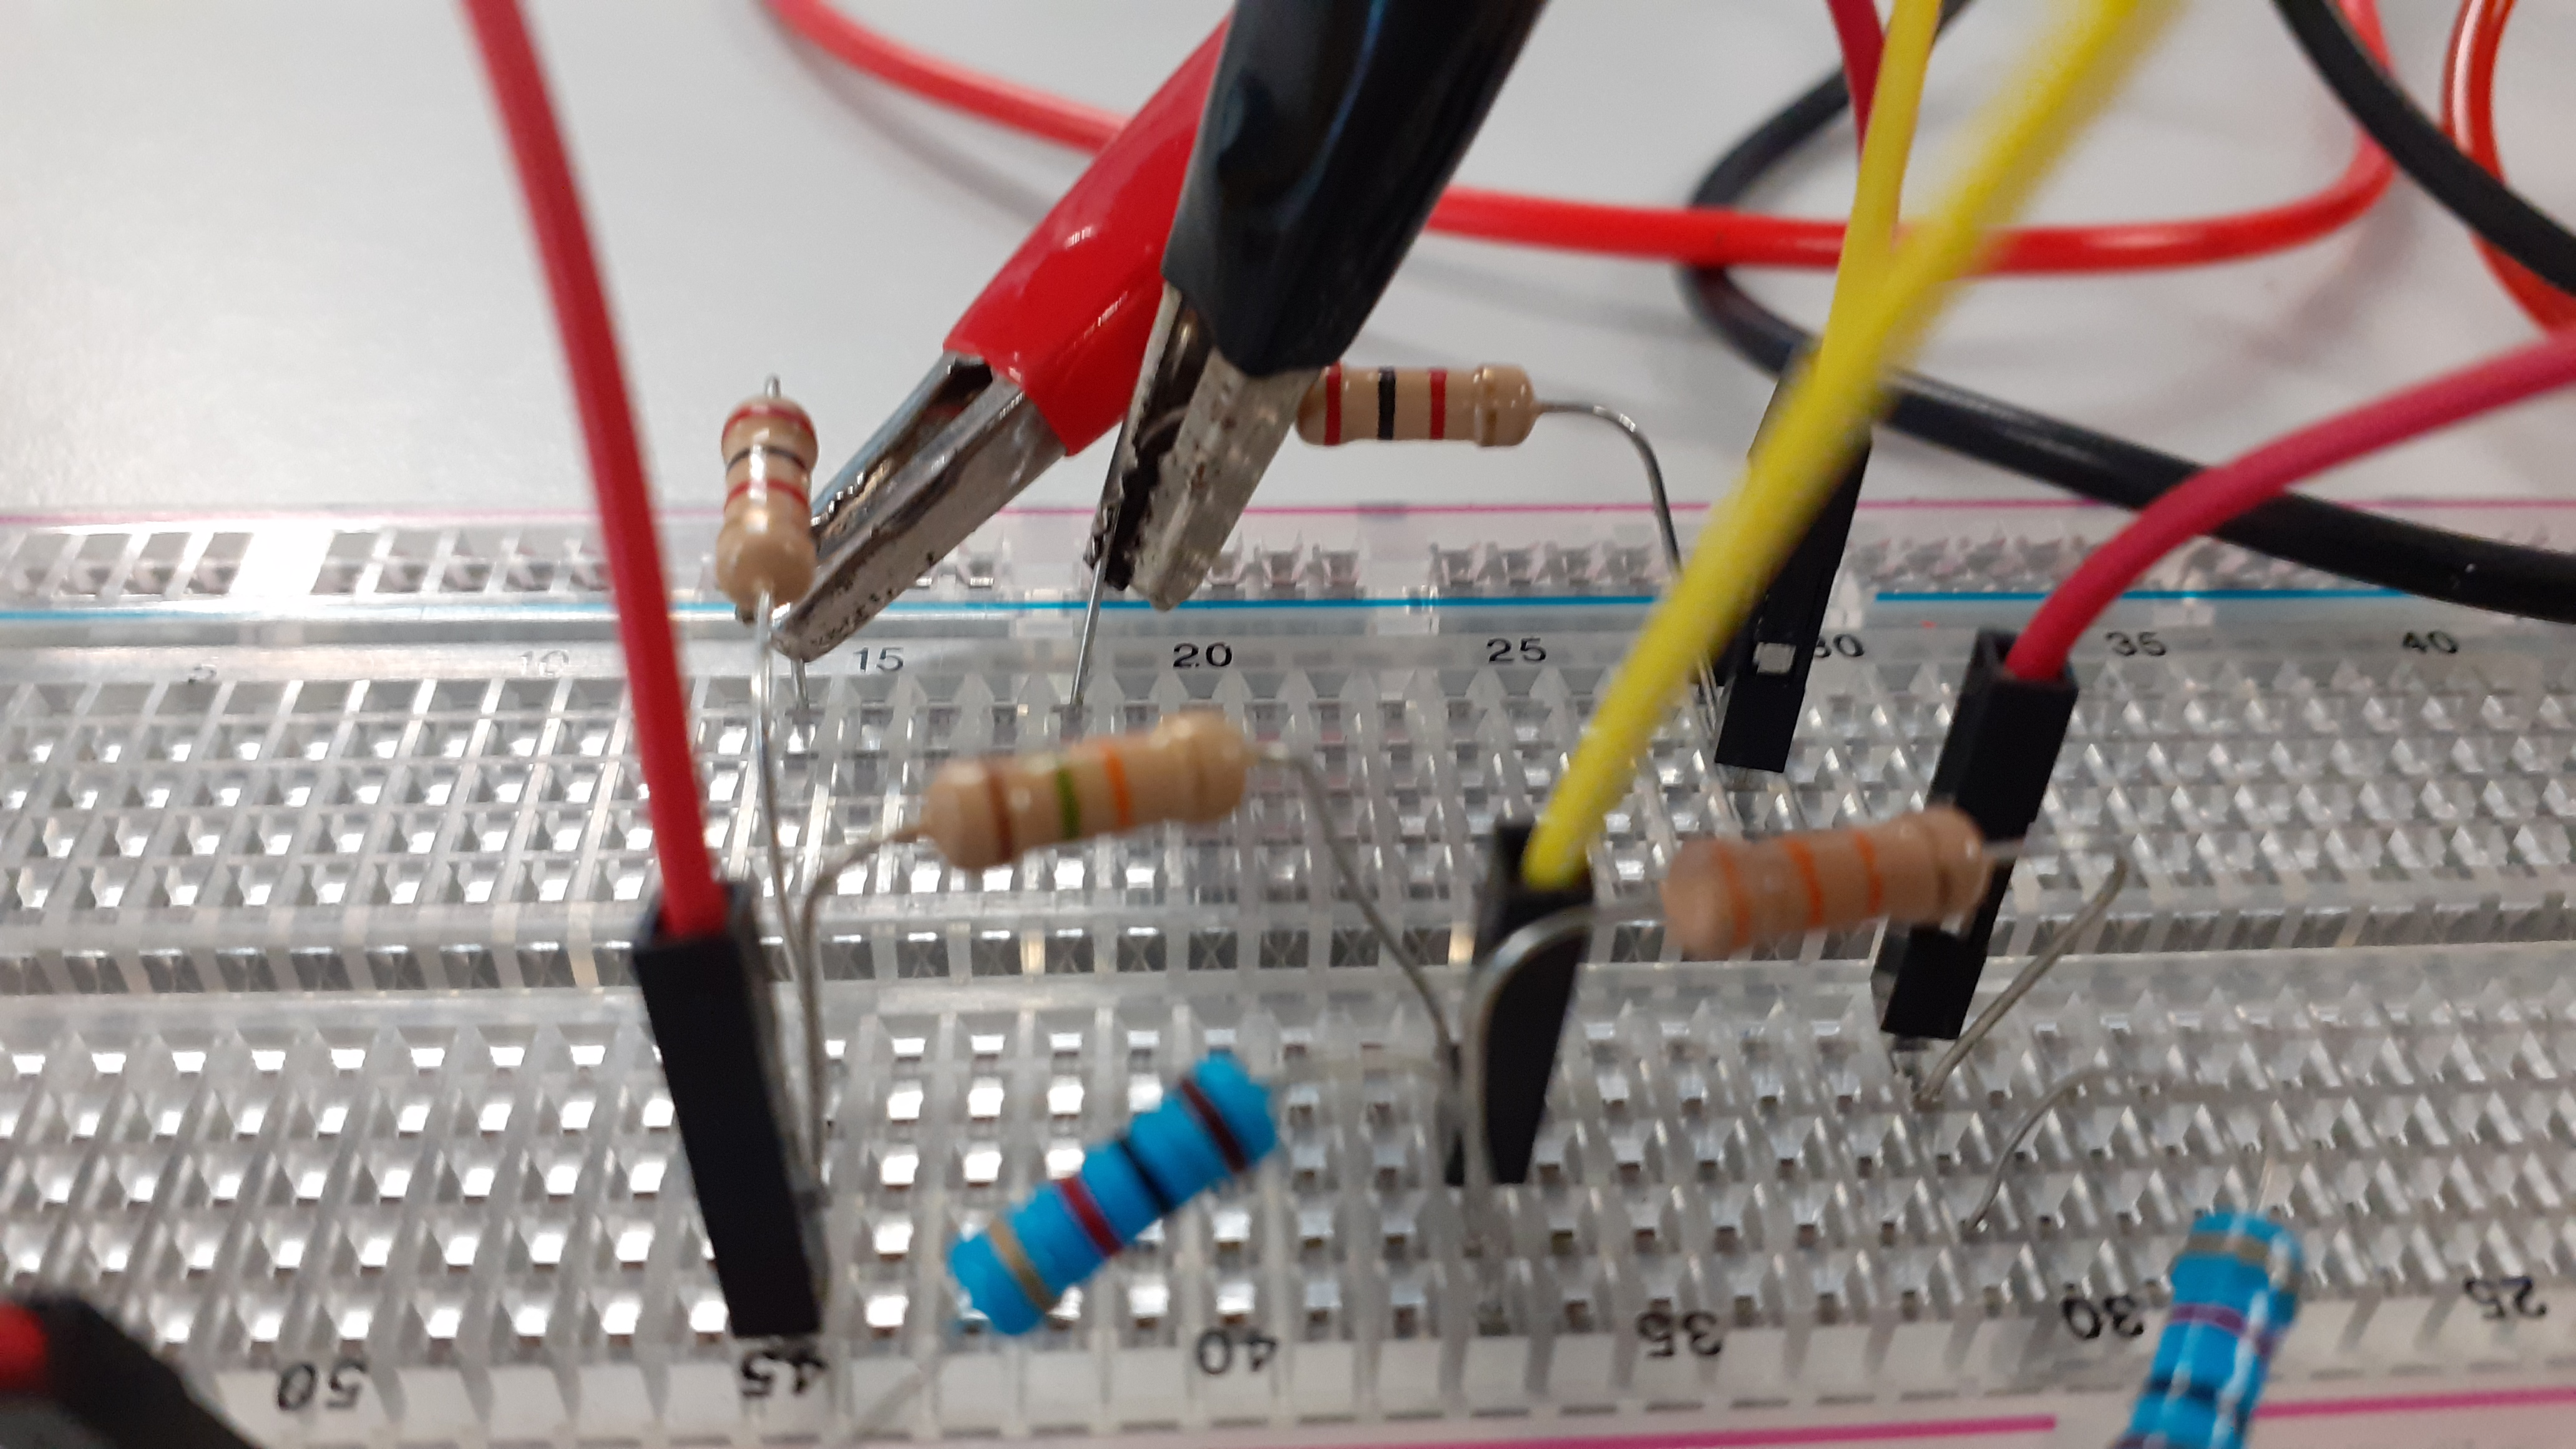
\includegraphics[width=0.9\linewidth]{20191108_093624}
		\caption{$A_2$}%
		\label{fig:a2}
	\end{subfigure}
\end{figure}
% }}}

% Circuito 1 {{{
\begin{figure}[H]
	\centering
	\begin{tikzpicture}
	[
		circuit ee IEC,
		set resistor graphic=var resistor IEC graphic
	]
	\boldmath

	\draw (0,0)
		to[battery={pos=0.3, info'=$9V$}]
		++(6,0);

	\draw (4,0)
		to[resistor={info'=$1k\Omega$}]
		++(0,2);

	\draw (6,0)
		to[resistor={info'=$1k\Omega$}]
		++(0,2);

	\draw (0,2)
		to
		[
			resistor={pos=0.4, info=$15k\Omega$},
			resistor={pos=((4+6)/12), info=$\cancel{33\Omega}$}
		]
		++(6,0);

	\draw (4,2) -- (6,4);

	\draw (6,2) -- ++(0,2)
		to
		[
			resistor={pos=0.25, info'=$10k\Omega$},
			resistor={pos=0.75, info'=$2k\Omega$}
		]
		++(-6,0)
		to[resistor={info'=$2k\Omega$}]
		++(0,-2)
		-- (0,0);

	\end{tikzpicture}
\end{figure}
% }}}
% Circuito 2 {{{
\begin{figure}[H]
	\centering
	\begin{tikzpicture}
	[
		circuit ee IEC,
		set resistor graphic=var resistor IEC graphic
	]
	\boldmath

	\draw (0,0)
		to
		[
			current direction' = {pos=0.1, info'=$I_1$},
			battery            = {pos=0.3, info'=$9V$},
			current direction' = {pos=0.9, info'=$I_6$}
		]
		++(6,0);

	\draw (4,0)
		to
		[
			resistor           = {info'=$1k\Omega$},
			current direction' = {pos=0.85, info'=$I_4$}
		]
		++(0,2);

	\draw (6,0)
		to[resistor={info'=$1k\Omega$}]
		++(0,2);

	\draw (0,2)
		to
		[
			current direction = {pos=0.2, info'=$I_3$},
			resistor          = {pos=0.4, info=$15k\Omega$},
			current direction = {pos=0.8, info=$I_5$}
		]
		++(6,0);

	\draw (6,2) -- ++(0,2)
		to
		[
			resistor           = {pos=0.25, info'=$10k\Omega$},
			current direction' = {pos=0.5, info'=$I_2$},
			resistor           = {pos=0.75, info'=$2k\Omega$}
		]
		++(-6,0)
		to[resistor={info'=$2k\Omega$}]
		++(0,-2)
		-- (0,0);

	\end{tikzpicture}
\end{figure}
% }}}

% Ecuaciones {{{
\begin{align*}
	I_1 &= I_2 + I_3\\
	I_3 &= I_4 + I_5\\
	I_6 &= I_2 + I_5\\
	%I_1 &= I_4 + I_6\\
	\\
	9 &= 14000I_2 + 1000I_6\\
	9 &= 15000I_3 + 1000I_6\\
	9 &= 15000I_3 + 1000I_4\\
	\\
	I_1 &= \frac{261}{224500}A\\
	I_2 &= \frac{27}{44900}A\\
	I_3 &= \frac{63}{112250}A\\
	I_4 &= \frac{261}{449000}A\\
	I_5 &= \frac{-9}{449000}A\\
	I_6 &= \frac{261}{449000}A
\end{align*}
% }}}

% Tabla {{{
\begin{table}[H]
	\centering
	\begin{tabular}{|c|c|c|c|}
		\hline
		Mediciones o lecturas de instrumentos & Teórico &
		\(
			\overset
			{
				(V:20V)(A:20mA)
			}
			{
				\text{Expermiental}
			}
		\)
		& Porcentaje de error\\
		\hline
		Lectura del amperímetro $A_1(I_1)$ &
		$1.16mA$ & $2.47$ &
		$\frac{|1.16-2.47|}{1.16}*100\%=112.93\%$
		\\
		\hline
		Corriente en la resistencia de $5k\Omega$ &
		\multicolumn{3}{c|}{No existe}\\
		\hline
		Lectura del amperímetro $A_2(I_2)$ &
		$0.6mA$ & $1.94$ &
		$\frac{|0.6-1.94|}{0.6}*100\%=223.33\%$\\
		\hline
		Corriente en la resistencia de $10k\Omega(I_2)$ &
		$0.6mA$ & $1.94$ &
		$\frac{|0.6-1.94|}{0.6}*100\%=223.33\%$\\
		\hline
		Lectura del amperímetro $A_3(I_6)$ &
		$0.58mA$ & $1.21$ &
		$\frac{|0.58-1.21|}{0.58}*100\%=108.62\%$\\
		\hline
		Voltaje en la resistencia de $30k\Omega$ &
		\multicolumn{3}{c|}{No existe}\\
		\hline
		Lectura del voltímetro $V_1$ &
		$0.58V$ & $1.23$ &
		$\frac{|0.58-1.23|}{0.58}*100\%=112.07\%$\\
		\hline
		Lectura del voltímetro $V_2$ &
		$1.20V$ & $3.92$ &
		$\frac{|1.20-3.92|}{1.20}*100\%=226.67\%$\\
		\hline
	\end{tabular}
\end{table}
% }}}

\end{document}
%}}}
